\section{Resultat}
\subsection{System 1}
Den analytiska lösningen för system 1 är
\begin{equation*}
    \begin{cases}
        x=\frac{27}{46}\cos(\frac{\sqrt{53}x}{5})+\sqrt{53}\sin(\frac{-\sqrt{53}x}{5})+\\
        \qquad\frac{-19}{46\sqrt{53}}(\sqrt{53}\cos(\frac{\sqrt{53}x}{5})+27\sin(\frac{-\sqrt{53}x}{5})\\
        \\[-7.5pt]
        y=\cos(\frac{\sqrt{53}}{5}t)+\frac{-19}{\sqrt{53}}\sin(\frac{-\sqrt{53}}{5}t)
    \end{cases}
\end{equation*}. En graf över olika steglängder och de associerade felen finnes i figur \ref{fig:diagram_sys_1_errors}.

\begin{figure}[h!]
    \centering
    % Automatically generated code. github.com/ohman-emil/GA
\begin{tikzpicture}
\definecolor{clr0}{RGB}{0, 114, 189}
\definecolor{clr1}{RGB}{217, 83, 25}
\definecolor{clr2}{RGB}{237, 177, 32}
\definecolor{clr3}{RGB}{126, 47, 142}
\definecolor{clr4}{RGB}{119, 172, 48}
\definecolor{clr5}{RGB}{77, 190, 238}
\definecolor{clr6}{RGB}{162, 20, 47}
\definecolor{clr7}{RGB}{120, 120, 120}
\begin{axis}[xmode=log,ymode=log,xlabel=Steglängd,ylabel=Avvikelse,width=\textwidth,height=0.6\textwidth,grid=both,minor grid style={draw=gray!33},major grid style={draw=gray},legend pos=south east,legend columns=2,legend style={column sep=1.5ex},]
\addplot[line width=1pt,mark=*,color=clr0] table {
0.05 1.6750755792762828
0.025 1.6836670243033418
0.0125 1.6438159414201832
0.00625 1.4104628232068364
0.003125 1.0016101885757394
0.0015625 0.6110836745847075
0.00078125 0.3395972996811829
0.000390625 0.17929090939529457
};
\addlegendentry{\hspace{{-1.25ex}}Euler 1}
\addplot[line width=1pt,mark=*,color=clr1] table {
0.05 2.5385976912679484
0.025 2.5788057118256185
0.0125 2.5327536079228596
0.00625 2.177537353746312
0.003125 1.5449812852953864
0.0015625 0.9412778612469512
0.00078125 0.522562409122171
0.000390625 0.27572173340265005
};
\addlegendentry{\hspace{{-1.25ex}}Euler 2}
\addplot[line width=1pt,mark=*,color=clr2] table {
0.05 0.009094604916475069
0.025 0.0016945605347229442
0.0125 0.000344297433158669
0.00625 7.571383342752647e-05
0.003125 1.760560197339167e-05
0.0015625 4.23430494400634e-06
0.00078125 1.0375805974405239e-06
0.000390625 2.567638994754873e-07
};
\addlegendentry{\hspace{{-1.25ex}}Heun 1}
\addplot[line width=1pt,mark=*,color=clr3] table {
0.05 0.03271401808365315
0.025 0.0073081808942934146
0.0125 0.001706531440970327
0.00625 0.00041079809817334834
0.003125 0.00010067098463961699
0.0015625 2.491107442459395e-05
0.00078125 6.195489655524966e-06
0.000390625 1.5448252912442229e-06
};
\addlegendentry{\hspace{{-1.25ex}}Heun 2}
\end{axis}
\end{tikzpicture}
    \caption{Avvikelsen i system 1 för de olika funktionerna.}
    \label{fig:diagram_sys_1_errors}
\end{figure}

\subsection{System 2}
Den analytiska lösningen för system 2 är
\begin{equation*}
    \begin{cases}
        x=(\frac{-36}{71}\cos(\frac{\sqrt{31}t}{5})-\frac{2\sqrt{31}}{71}\sin(\frac{\sqrt{31}t}{5}))+\\
        \qquad \frac{107}{142\sqrt{31}}(2\sqrt{31}\cos(\frac{\sqrt{31}t}{5})-36\sin(\frac{\sqrt{31}t}{5}))\\
        \\[-7.5pt]
        y=\cos({\frac{\sqrt{31}t}{5}})+\frac{107}{2\sqrt{31}}\sin(\frac{\sqrt{31}t}{5})
    \end{cases}
\end{equation*}. En graf över olika steglängder och de associerade felen finnes i figur \ref{fig:diagram_sys_2_errors}.

\begin{figure}[h!]
    \centering
    % Automatically generated code. github.com/ohman-emil/GA
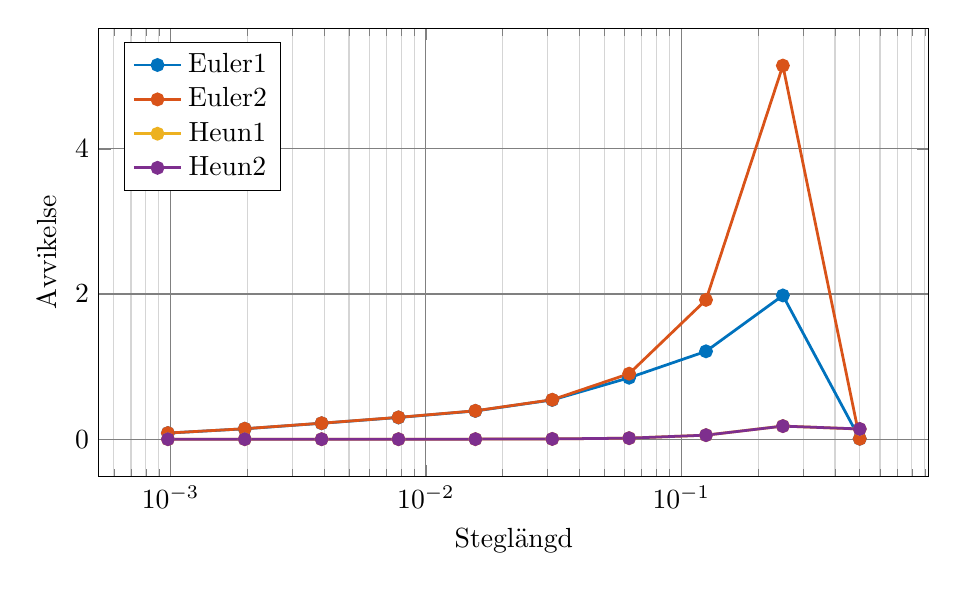
\begin{tikzpicture}
\definecolor{clr0}{RGB}{0, 114, 189}
\definecolor{clr1}{RGB}{217, 83, 25}
\definecolor{clr2}{RGB}{237, 177, 32}
\definecolor{clr3}{RGB}{126, 47, 142}
\definecolor{clr4}{RGB}{119, 172, 48}
\definecolor{clr5}{RGB}{77, 190, 238}
\definecolor{clr6}{RGB}{162, 20, 47}
\begin{axis}[xmode=log,xlabel=Steglängd,ylabel=Avvikelse,width=\textwidth,height=0.6\textwidth,grid=both,minor grid style={draw=gray!33},major grid style={draw=gray},legend pos=north west,]
\addplot[line width=1pt,mark=*,color=clr0,] table {
0.5 0.005989385117099618
0.25 1.9803649785603574
0.125 1.2107783484306052
0.0625 0.8465263250289623
0.03125 0.5406037712531494
0.015625 0.38928393239226483
0.0078125 0.2992813458164704
0.00390625 0.21934673899985133
0.001953125 0.143394626093829
0.0009765625 0.08413747164826592
};
\addlegendentry{Euler1}
\addplot[line width=1pt,mark=*,color=clr1,] table {
0.5 0.005989385117099618
0.25 5.147474617589516
0.125 1.9193045168161569
0.0625 0.9025180073753696
0.03125 0.5438634090216116
0.015625 0.39140776613968403
0.0078125 0.3009530155769476
0.00390625 0.22072242869212985
0.001953125 0.14440828338510722
0.0009765625 0.08478161923291445
};
\addlegendentry{Euler2}
\addplot[line width=1pt,mark=*,color=clr2,] table {
0.5 0.13968683273538496
0.25 0.18106701393818045
0.125 0.05597526368112834
0.0625 0.014324774152084075
0.03125 0.0035920397966477577
0.015625 0.0008983445576930589
0.0078125 0.00022459685621547358
0.00390625 5.6149609174212024e-05
0.001953125 1.4037405951053175e-05
0.0009765625 3.50934979237587e-06
};
\addlegendentry{Heun1}
\addplot[line width=1pt,mark=*,color=clr3,] table {
0.5 0.14098811929408778
0.25 0.18028388662134673
0.125 0.055723539632161305
0.0625 0.014284112858846256
0.03125 0.003580080314228922
0.015625 0.0008952821264982448
0.0078125 0.00022381574510458782
0.00390625 5.5952065218473914e-05
0.001953125 1.3987723154916891e-05
0.0009765625 3.49689115384739e-06
};
\addlegendentry{Heun2}
\end{axis}
\end{tikzpicture}
    \caption{Avvikelsen i system 2 för de olika funktionerna.}
    \label{fig:diagram_sys_2_errors}
\end{figure}

\subsection{System 3}
Den analytiska lösningen för system 3 är
\begin{equation*}
    \begin{cases}
        x=(\frac{78}{73}\cos(\frac{\sqrt{231}t}{5})-\frac{2\sqrt{231}}{73}\sin(\frac{\sqrt{231}t}{5})-\\
        \qquad \frac{5}{2\sqrt{231}}(\frac{2\sqrt{231}}{73}\cos(\frac{\sqrt{231}t}{5})-\frac{78}{73}\sin(\frac{\sqrt{231}t}{5}))\\
        \\[-7.5pt]
        y=\cos({\frac{\sqrt{231}t}{5}})-\frac{5}{2\sqrt{231}}\sin(\frac{\sqrt{231}t}{5})
    \end{cases}
\end{equation*}. En graf över olika steglängder och de associerade felen finnes i figur \ref{fig:diagram_sys_3_errors}.

\begin{figure}[h!]
    \centering
    % Automatically generated code. github.com/ohman-emil/GA
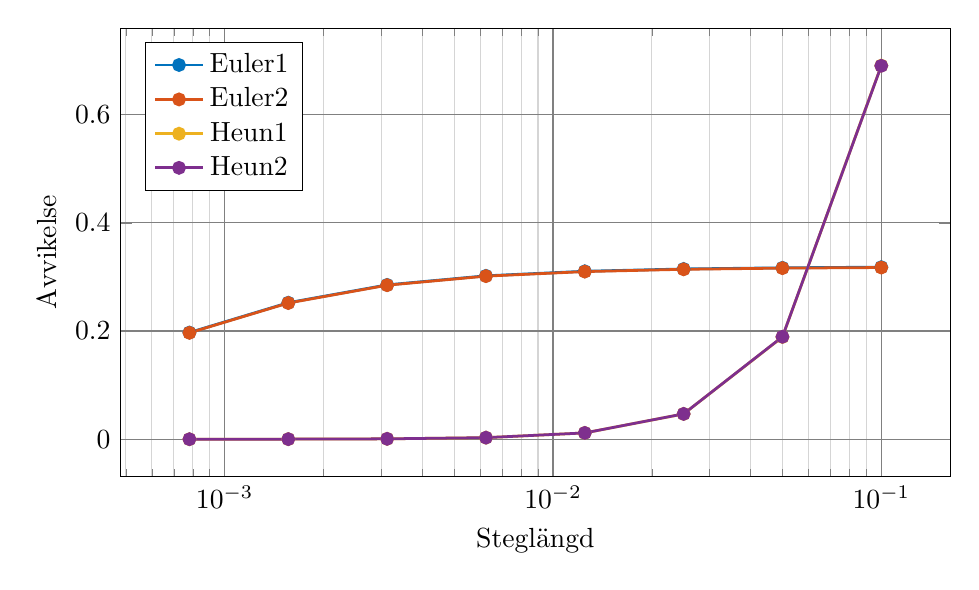
\begin{tikzpicture}
\definecolor{clr0}{RGB}{0, 114, 189}
\definecolor{clr1}{RGB}{217, 83, 25}
\definecolor{clr2}{RGB}{237, 177, 32}
\definecolor{clr3}{RGB}{126, 47, 142}
\definecolor{clr4}{RGB}{119, 172, 48}
\definecolor{clr5}{RGB}{77, 190, 238}
\definecolor{clr6}{RGB}{162, 20, 47}
\begin{axis}[xmode=log,xlabel=Steglängd,ylabel=Avvikelse,width=\textwidth,height=0.6\textwidth,grid=both,minor grid style={draw=gray!33},major grid style={draw=gray},legend pos=north west,]
\addplot[line width=1pt,mark=*,color=clr0,] table {
0.1 0.3180672011264721
0.05 0.3168591926193936
0.025 0.3147073783975929
0.0125 0.3104597995273267
0.00625 0.3020432537496696
0.003125 0.28527247317974963
0.0015625 0.2523397682455023
0.00078125 0.1971863324001217
};
\addlegendentry{Euler1}
\addplot[line width=1pt,mark=*,color=clr1,] table {
0.1 0.31734682752647586
0.05 0.31623840858637176
0.025 0.3140815082460575
0.0125 0.3098496175647469
0.00625 0.301444834418717
0.003125 0.2846828798039043
0.0015625 0.2517605494767164
0.00078125 0.19665880546425718
};
\addlegendentry{Euler2}
\addplot[line width=1pt,mark=*,color=clr2,] table {
0.1 0.6906295663697244
0.05 0.18898871842982973
0.025 0.0467711168348623
0.0125 0.011660962086257746
0.00625 0.0029140638556928032
0.003125 0.0007284765486063044
0.0015625 0.00018211732427183722
0.00078125 4.552915897118063e-05
};
\addlegendentry{Heun1}
\addplot[line width=1pt,mark=*,color=clr3,] table {
0.1 0.6902373549189035
0.05 0.18938087144039725
0.025 0.04682253912693223
0.0125 0.011671262944273035
0.00625 0.0029165933364919006
0.003125 0.0007291216041849388
0.0015625 0.00018228127933073537
0.00078125 4.557055178802054e-05
};
\addlegendentry{Heun2}
\end{axis}
\end{tikzpicture}
    \caption{Avvikelsen i system 3 för de olika funktionerna.}
    \label{fig:diagram_sys_3_errors}
\end{figure}

\subsection{System 4}
Den analytiska lösningen för system 4 är
\begin{equation*}
    \begin{cases}
        x=(\frac{20}{26}\cos(\frac{\sqrt{\frac{1}{2}203}t}{5})+\frac{\sqrt{406}}{26}\sin(\frac{\sqrt{\frac{1}{2}203}t}{5}))-\\
        \qquad \frac{6}{\sqrt{406}}(\frac{-\sqrt{406}}{26}\cos(\frac{\sqrt{\frac{1}{2}203}t}{5})-\frac{20}{26}\sin(\frac{\sqrt{\frac{1}{2}203}t}{5}))\\
        \\[-7.5pt]
        y=\cos({\frac{\sqrt{\frac{1}{2}203}t}{5}})+\frac{107}{2\sqrt{31}}\sin(\frac{\sqrt{\frac{1}{2}203}t}{5})
    \end{cases}
\end{equation*}. En graf över olika steglängder och de associerade felen finnes i figur \ref{fig:diagram_sys_4_errors}.

\begin{figure}[h!]
    \centering
    % Automatically generated code. github.com/ohman-emil/GA
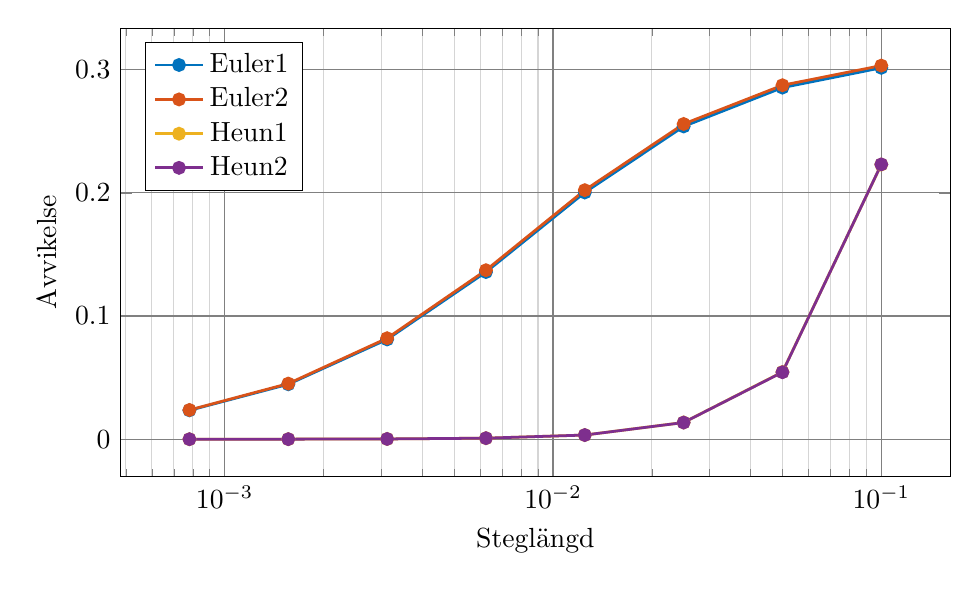
\begin{tikzpicture}
\definecolor{clr0}{RGB}{0, 114, 189}
\definecolor{clr1}{RGB}{217, 83, 25}
\definecolor{clr2}{RGB}{237, 177, 32}
\definecolor{clr3}{RGB}{126, 47, 142}
\definecolor{clr4}{RGB}{119, 172, 48}
\definecolor{clr5}{RGB}{77, 190, 238}
\definecolor{clr6}{RGB}{162, 20, 47}
\begin{axis}[xmode=log,xlabel=Steglängd,ylabel=Avvikelse,width=\textwidth,height=0.6\textwidth,grid=both,minor grid style={draw=gray!33},major grid style={draw=gray},legend pos=north west,]
\addplot[line width=1pt,mark=*,color=clr0,] table {
0.1 0.3014217025698702
0.05 0.28535571954917016
0.025 0.25385222750846853
0.0125 0.2002469657423705
0.00625 0.13567742220816262
0.003125 0.08100449807733635
0.0015625 0.04458015866832087
0.00078125 0.02343025533076309
};
\addlegendentry{Euler1}
\addplot[line width=1pt,mark=*,color=clr1,] table {
0.1 0.30323856267060917
0.05 0.2872837889203839
0.025 0.25584992828308717
0.0125 0.20213266161334004
0.00625 0.13715549659635248
0.003125 0.08196981851425594
0.0015625 0.04513818779319952
0.00078125 0.02373112935746454
};
\addlegendentry{Euler2}
\addplot[line width=1pt,mark=*,color=clr2,] table {
0.1 0.22292054450235077
0.05 0.05456144568498825
0.025 0.013581861039854839
0.0125 0.0033933164498776533
0.00625 0.0008482401567670911
0.003125 0.00021205330768014097
0.0015625 5.3012484531435475e-05
0.00078125 1.3253007721488278e-05
};
\addlegendentry{Heun1}
\addplot[line width=1pt,mark=*,color=clr3,] table {
0.1 0.22304780706060093
0.05 0.05437175713392498
0.025 0.013526481590799576
0.0125 0.0033794625521774255
0.00625 0.0008448358649512316
0.003125 0.00021121338881513707
0.0015625 5.2804170683412734e-05
0.00078125 1.32011532978316e-05
};
\addlegendentry{Heun2}
\end{axis}
\end{tikzpicture}
    \caption{Avvikelsen i system 4 för de olika funktionerna.}
    \label{fig:diagram_sys_4_errors}
\end{figure}

\subsection{System 5}
Den analytiska lösningen för system 5 är
\begin{equation*}
    \begin{cases}
        x=\frac{2416}{2371}(\frac{-23}{58}\cos(\frac{\sqrt{2371}t}{10})+\frac{\sqrt{2371}}{58}\sin(\frac{\sqrt{2371}t}{10}))-\\
        \qquad \frac{16}{\sqrt{2371}}(\frac{-\sqrt{2371}}{58}\cos(\frac{\sqrt{2371}t}{10})+\frac{23}{58}\sin(\frac{\sqrt{2371}t}{10}))+\frac{2675}{2371}\\
        \\[-7.5pt]
        y=\frac{2416}{2371}\cos(\frac{\sqrt{2371}t}{10})-\frac{+16}{\sqrt{2371}}\sin(\frac{\sqrt{2371}t}{10})-\frac{45}{2371}
    \end{cases}
\end{equation*}. Den motsvarande homogena differentialekvationen har lösningen 
\begin{equation*}
    \begin{cases}
        x=(\frac{-23}{58}\cos(\frac{\sqrt{2371}t}{10})+\frac{+\sqrt{2371}}{58}\sin(\frac{\sqrt{2371}t}{10}))-\\
        \qquad \frac{81}{\sqrt{2371}}(\frac{-\sqrt{2371}}{58}\cos(\frac{\sqrt{2371}t}{10})-\frac{-23}{58}\sin(\frac{\sqrt{2371}t}{10}))\\
        \\[-7.5pt]
        y=\cos(\frac{\sqrt{2371}t}{10})-\frac{81}{\sqrt{2371}}\sin(\frac{\sqrt{2371}t}{10})
    \end{cases}
\end{equation*}. En graf över olika steglängder och de associerade felen finnes i figur \ref{fig:diagram_sys_5_errors}.

\begin{figure}[h!]
    \centering

    \begin{subfigure}[h]{\textwidth}
        % Automatically generated code. github.com/ohman-emil/GA
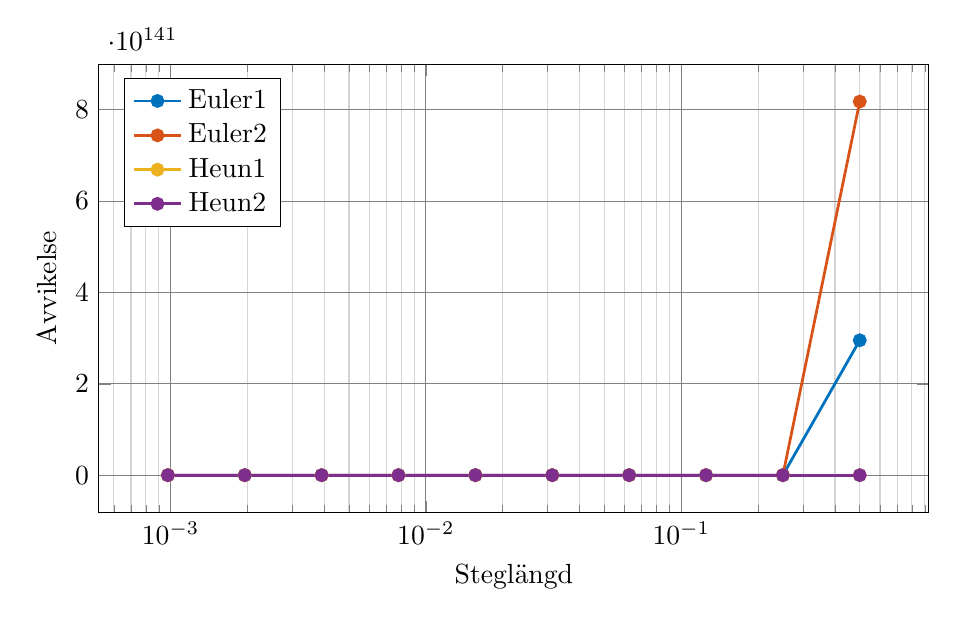
\begin{tikzpicture}
\definecolor{clr0}{RGB}{0, 114, 189}
\definecolor{clr1}{RGB}{217, 83, 25}
\definecolor{clr2}{RGB}{237, 177, 32}
\definecolor{clr3}{RGB}{126, 47, 142}
\definecolor{clr4}{RGB}{119, 172, 48}
\definecolor{clr5}{RGB}{77, 190, 238}
\definecolor{clr6}{RGB}{162, 20, 47}
\begin{axis}[xmode=log,xlabel=Steglängd,ylabel=Avvikelse,width=\textwidth,height=0.6\textwidth,grid=both,minor grid style={draw=gray!33},major grid style={draw=gray},legend pos=north west,]
\addplot[line width=1pt,mark=*,color=clr0,] table {
0.5 2.9524953778948422e+141
0.25 0.3167381985006317
0.125 0.30920293404134236
0.0625 0.2984074749081066
0.03125 0.27854828190558645
0.015625 0.24093298245438408
0.0078125 0.18221020057423795
0.00390625 0.11867892442296757
0.001953125 0.06897143705773831
0.0009765625 0.03736779649764003
};
\addlegendentry{Euler1}
\addplot[line width=1pt,mark=*,color=clr1,] table {
0.5 8.17817951512437e+141
0.25 0.32054295294251367
0.125 0.3122503019125455
0.0625 0.29944624330903635
0.03125 0.2785612200769082
0.015625 0.24044819211722657
0.0078125 0.18156804978113145
0.00390625 0.11813784462917352
0.001953125 0.06861487391059849
0.0009765625 0.03716220430862328
};
\addlegendentry{Euler2}
\addplot[line width=1pt,mark=*,color=clr2,] table {
0.5 8.893218770685648e+95
0.25 3.08312729811997e+35
0.125 16983.513903618365
0.0625 0.848390293494165
0.03125 0.29867887721661374
0.015625 0.07517023069112065
0.0078125 0.01872676993884599
0.00390625 0.004678531403668692
0.001953125 0.0011695389576915954
0.0009765625 0.0002923851122200028
};
\addlegendentry{Heun1}
\addplot[line width=1pt,mark=*,color=clr3,] table {
0.5 1.0912240774133727e+96
0.25 3.537597035239887e+35
0.125 16806.2827350711
0.0625 0.8473270588476569
0.03125 0.2986029778926087
0.015625 0.07500551189131384
0.0078125 0.018684370828993584
0.00390625 0.004667935904350018
0.001953125 0.001166890531406937
0.0009765625 0.00029172299759632874
};
\addlegendentry{Heun2}
\end{axis}
\end{tikzpicture}
        \caption{Homogen}
    \end{subfigure}
    %
    \vspace{1em}\newline
    %
    \begin{subfigure}[h]{\textwidth}
        % Automatically generated code. github.com/ohman-emil/GA
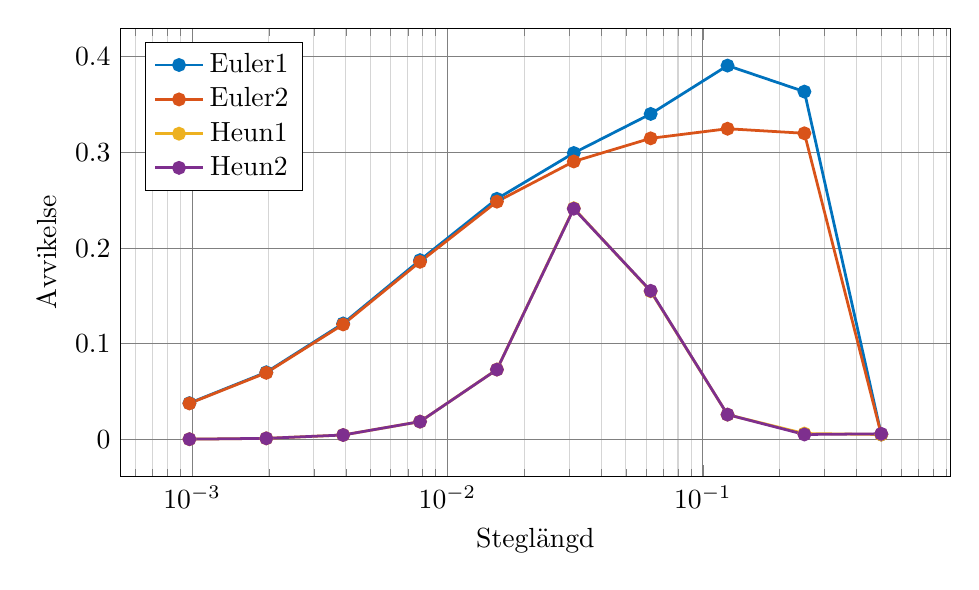
\begin{tikzpicture}
\definecolor{clr0}{RGB}{0, 114, 189}
\definecolor{clr1}{RGB}{217, 83, 25}
\definecolor{clr2}{RGB}{237, 177, 32}
\definecolor{clr3}{RGB}{126, 47, 142}
\definecolor{clr4}{RGB}{119, 172, 48}
\definecolor{clr5}{RGB}{77, 190, 238}
\definecolor{clr6}{RGB}{162, 20, 47}
\begin{axis}[xmode=log,xlabel=Steglängd,ylabel=Avvikelse,width=\textwidth,height=0.6\textwidth,grid=both,minor grid style={draw=gray!33},major grid style={draw=gray},legend pos=north west,]
\addplot[line width=1pt,mark=*,color=clr0,] table {
0.5 0.005183797768440612
0.25 0.36351413446567327
0.125 0.3907155410563677
0.0625 0.3401989180765902
0.03125 0.29937805955905616
0.015625 0.25146609389318314
0.0078125 0.18739930070321634
0.00390625 0.12123160190530245
0.001953125 0.07022895348263794
0.0009765625 0.037990548636016835
};
\addlegendentry{Euler1}
\addplot[line width=1pt,mark=*,color=clr1,] table {
0.5 0.005183797768440612
0.25 0.3199600902467052
0.125 0.3247258584794036
0.0625 0.3146892421581639
0.03125 0.29052267950915045
0.015625 0.24852901693706544
0.0078125 0.185667456554958
0.00390625 0.12020466066162167
0.001953125 0.06965331316905986
0.0009765625 0.03768295652253027
};
\addlegendentry{Euler2}
\addplot[line width=1pt,mark=*,color=clr2,] table {
0.5 0.005186597467347092
0.25 0.006198737450916862
0.125 0.02594959175472362
0.0625 0.15487782325335148
0.03125 0.24162225863224665
0.015625 0.07310374091547733
0.0078125 0.018638310589407944
0.00390625 0.004669660736641595
0.001953125 0.0011677390563065771
0.0009765625 0.0002919489175417706
};
\addlegendentry{Heun1}
\addplot[line width=1pt,mark=*,color=clr3,] table {
0.5 0.005905550981178217
0.25 0.005209031803682314
0.125 0.025989026457246118
0.0625 0.15532541113515821
0.03125 0.2411573949900024
0.015625 0.07301830642487864
0.0078125 0.01862620602621824
0.00390625 0.004667060735636622
0.001953125 0.0011670928180446739
0.0009765625 0.000291783188239929
};
\addlegendentry{Heun2}
\end{axis}
\end{tikzpicture}
        \caption{Inhomogen}
    \end{subfigure}

    \caption{Avvikelsen i system 5 för de olika funktionerna.}
    \label{fig:diagram_sys_5_errors}
\end{figure}

\subsection{System 6}
Den analytiska lösningen för system 6 är
\begin{equation*}
    \begin{cases}
        x=\frac{1194}{103}(\frac{-72}{55}\cos(\frac{\sqrt{\frac{1}{2}103}t}{5})+\frac{\sqrt{206}}{55}\sin(\frac{\sqrt{\frac{1}{2}103}t}{5}))-\\
        \qquad \frac{43\sqrt{206}}{103}(\frac{-\sqrt{206}}{55}\cos(\frac{\sqrt{\frac{1}{2}103}t}{5})+\frac{72}{55}\sin(\frac{\sqrt{\frac{1}{2}103}t}{5}))+\frac{1505}{103}\\
        \\[-7.5pt]
        y=\frac{1194}{103}\cos({\frac{\sqrt{\frac{1}{2}103}t}{5}})-\frac{43\sqrt{206}}{103}\sin(\frac{\sqrt{\frac{1}{2}103}t}{5})-\frac{1091}{103}
    \end{cases}
\end{equation*}. Den motsvarande homogena differentialekvationen har lösningen 
\begin{equation*}
    \begin{cases}
        x=(\frac{-72}{55}\cos(\frac{\sqrt{\frac{1}{2}103}t}{5})+\frac{\sqrt{206}}{55}\sin(\frac{\sqrt{\frac{1}{2}103}t}{5}))-\\
        \qquad \frac{127}{\sqrt{206}}(\frac{-\sqrt{206}}{55}\cos(\frac{\sqrt{\frac{1}{2}103}t}{5})+\frac{72}{55}\sin(\frac{\sqrt{\frac{1}{2}103}t}{5}))\\
        \\[-7.5pt]
        y=\cos({\frac{\sqrt{\frac{1}{2}103}t}{5}})-\frac{127}{\sqrt{206}}\sin(\frac{\sqrt{\frac{1}{2}103}t}{5})
    \end{cases}
\end{equation*}. En graf över olika steglängder och de associerade felen finnes i figur \ref{fig:diagram_sys_6_errors}.

\begin{figure}[h!]
    \centering

    \begin{subfigure}[h]{\textwidth}
        % Automatically generated code. github.com/ohman-emil/GA
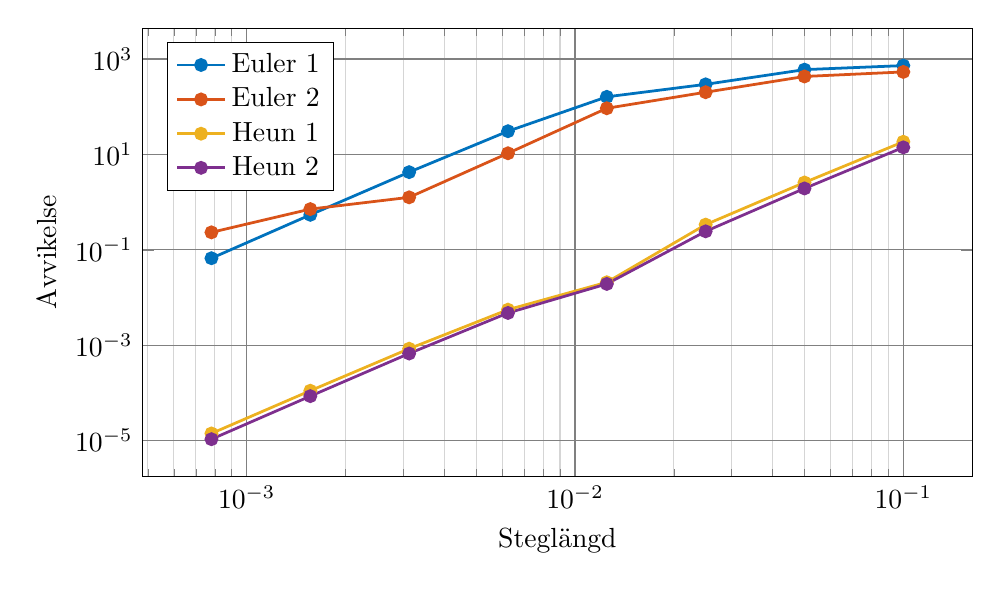
\begin{tikzpicture}
\definecolor{clr0}{RGB}{0, 114, 189}
\definecolor{clr1}{RGB}{217, 83, 25}
\definecolor{clr2}{RGB}{237, 177, 32}
\definecolor{clr3}{RGB}{126, 47, 142}
\definecolor{clr4}{RGB}{119, 172, 48}
\definecolor{clr5}{RGB}{77, 190, 238}
\definecolor{clr6}{RGB}{162, 20, 47}
\begin{axis}[xmode=log,ymode=log,xlabel=Steglängd,ylabel=Avvikelse,width=\textwidth,height=0.6\textwidth,grid=both,minor grid style={draw=gray!33},major grid style={draw=gray},legend pos=north west,]
\addplot[line width=1pt,mark=*,color=clr0] table {
0.1 728.782917316358
0.05 599.4770899575655
0.025 294.75437750751473
0.0125 161.23123894509473
0.00625 30.657014872267276
0.003125 4.246565083036572
0.0015625 0.5403589767551216
0.00078125 0.06654424815209636
};
\addlegendentry{Euler 1}
\addplot[line width=1pt,mark=*,color=clr1] table {
0.1 536.4730450691388
0.05 430.84864463375595
0.025 201.41440121215342
0.0125 92.80460552212948
0.00625 10.568622648295836
0.003125 1.2580098624521365
0.0015625 0.7129107481850188
0.00078125 0.2320796924746035
};
\addlegendentry{Euler 2}
\addplot[line width=1pt,mark=*,color=clr2] table {
0.1 18.405138906106114
0.05 2.574510634306033
0.025 0.3370121731740936
0.0125 0.02082705606944857
0.00625 0.005548458039600135
0.003125 0.0008416045323991206
0.0015625 0.00011075852439046407
0.00078125 1.4065161648924018e-05
};
\addlegendentry{Heun 1}
\addplot[line width=1pt,mark=*,color=clr3] table {
0.1 14.053409418292846
0.05 1.9315723391082273
0.025 0.2436781363996786
0.0125 0.0192245405200121
0.00625 0.004732733694065794
0.003125 0.0006677625851893854
0.0015625 8.521974713803643e-05
0.00078125 1.066287282832333e-05
};
\addlegendentry{Heun 2}
\end{axis}
\end{tikzpicture}
        \caption{Homogen}
    \end{subfigure}
    %
    \vspace{1em}\newline
    %
    \begin{subfigure}[h]{\textwidth}
        % Automatically generated code. github.com/ohman-emil/GA
\begin{tikzpicture}
\definecolor{clr0}{RGB}{0, 114, 189}
\definecolor{clr1}{RGB}{217, 83, 25}
\definecolor{clr2}{RGB}{237, 177, 32}
\definecolor{clr3}{RGB}{126, 47, 142}
\definecolor{clr4}{RGB}{119, 172, 48}
\definecolor{clr5}{RGB}{77, 190, 238}
\definecolor{clr6}{RGB}{162, 20, 47}
\definecolor{clr7}{RGB}{120, 120, 120}
\begin{axis}[xmode=log,ymode=log,xlabel=Steglängd,ylabel=Avvikelse,width=\textwidth,height=0.6\textwidth,grid=both,minor grid style={draw=gray!33},major grid style={draw=gray},legend pos=south east,legend columns=2,legend style={column sep=1.5ex},]
\addplot[line width=1pt,mark=*,color=clr0] table {
0.05 8.920652440316031
0.025 8.37821064614715
0.0125 8.080022154182531
0.00625 7.540643557429654
0.003125 6.146659553213063
0.0015625 4.21939934468222
0.00078125 2.529523449987199
0.000390625 1.3937699851842922
};
\addlegendentry{\hspace{{-1.25ex}}Euler \(x\)}
\addplot[line width=1pt,mark=*,color=clr1] table {
0.05 8.745095388151844
0.025 8.392029280195224
0.0125 8.192976243131879
0.00625 7.730858061023643
0.003125 6.356695867801246
0.0015625 4.377524945480639
0.00078125 2.625418973858924
0.000390625 1.446247542990708
};
\addlegendentry{\hspace{{-1.25ex}}Euler \(y\)}
\addplot[line width=1pt,mark=*,color=clr2] table {
0.05 0.3584634792524355
0.025 0.09270020533766044
0.0125 0.023569793064847744
0.00625 0.005941880326357563
0.003125 0.0014916380668665852
0.0015625 0.00037367928450393606
0.00078125 9.351594833262311e-05
0.000390625 2.3390995316674434e-05
};
\addlegendentry{\hspace{{-1.25ex}}Heun \(x\)}
\addplot[line width=1pt,mark=*,color=clr3] table {
0.05 0.22902186327342378
0.025 0.06023122961111227
0.0125 0.015446320262398672
0.00625 0.003910860174180186
0.003125 0.000983908723071636
0.0015625 0.0002467531299537029
0.00078125 6.178537346812618e-05
0.000390625 1.545848440898112e-05
};
\addlegendentry{\hspace{{-1.25ex}}Heun \(y\)}
\end{axis}
\end{tikzpicture}
        \caption{Inhomogen}
    \end{subfigure}

    \caption{Avvikelsen i system 6 för de olika funktionerna.}
    \label{fig:diagram_sys_6_errors}
\end{figure}

\subsection{System 7}
Den analytiska lösningen för system 7 är
\begin{equation*}
    \begin{cases}
        x=\frac{739}{13}(\frac{-38}{35}\cos(\frac{\sqrt{26t}}{5})+\frac{\sqrt{26}}{35}\sin(\frac{\sqrt{26t}}{5}))-\\
        \qquad \frac{73}{\sqrt{26}}(\frac{\sqrt{26}}{35}\cos(\frac{\sqrt{26t}}{5})-\frac{38}{35}\sin(\frac{\sqrt{26t}}{5}))+\frac{1585}{26}\\
        \\[-7.5pt]
        y=\frac{739}{13}\cos(\frac{\sqrt{26t}}{5})+\frac{38}{35}\sin(\frac{\sqrt{26t}}{5})-\frac{726}{13}
    \end{cases}
\end{equation*}. Den motsvarande homogena differentialekvationen har lösningen 
\begin{equation*}
    \begin{cases}
        x=(\frac{-38}{35}\cos(\frac{\sqrt{26t}}{5})+\frac{\sqrt{26}}{35}\sin(\frac{\sqrt{26t}}{5}))-\\
        \qquad \frac{73}{\sqrt{26}}(\frac{\sqrt{26}}{35}\cos(\frac{\sqrt{26t}}{5})-\frac{38}{35}\sin(\frac{\sqrt{26t}}{5}))\\
        \\[-7.5pt]
        y=\cos(\frac{\sqrt{26t}}{5})+\frac{38}{35}\sin(\frac{\sqrt{26t}}{5})
    \end{cases}
\end{equation*}. En graf över olika steglängder och de associerade felen finnes i figur \ref{fig:diagram_sys_7_errors}.

\begin{figure}[h!]
    \centering

    \begin{subfigure}[h]{\textwidth}
        % Automatically generated code. github.com/ohman-emil/GA
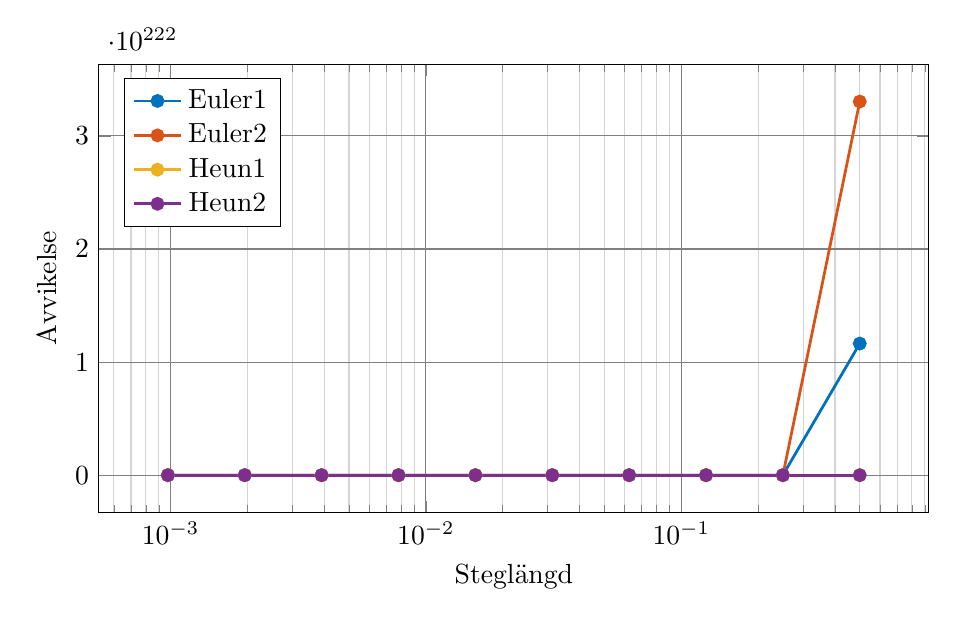
\begin{tikzpicture}
\definecolor{clr0}{RGB}{0, 114, 189}
\definecolor{clr1}{RGB}{217, 83, 25}
\definecolor{clr2}{RGB}{237, 177, 32}
\definecolor{clr3}{RGB}{126, 47, 142}
\definecolor{clr4}{RGB}{119, 172, 48}
\definecolor{clr5}{RGB}{77, 190, 238}
\definecolor{clr6}{RGB}{162, 20, 47}
\begin{axis}[xmode=log,xlabel=Steglängd,ylabel=Avvikelse,width=\textwidth,height=0.6\textwidth,grid=both,minor grid style={draw=gray!33},major grid style={draw=gray},legend pos=north west,]
\addplot[line width=1pt,mark=*,color=clr0,] table {
0.5 1.163951087535368e+222
0.25 3.1016961353130932e+165
0.125 0.31691857215907826
0.0625 0.3161883512666636
0.03125 0.31452513559293094
0.015625 0.3110626910926746
0.0078125 0.30404372212791714
0.00390625 0.2899540401371384
0.001953125 0.2619454960920262
0.0009765625 0.21204905903490034
};
\addlegendentry{Euler1}
\addplot[line width=1pt,mark=*,color=clr1,] table {
0.5 3.3039740081905977e+222
0.25 2.8431396600483566e+165
0.125 0.31756181968203234
0.0625 0.3168205427010895
0.03125 0.31515884201130134
0.015625 0.31170183444905397
0.0078125 0.30468767344165937
0.00390625 0.2906011965636223
0.001953125 0.2625924717637946
0.0009765625 0.21266087313971796
};
\addlegendentry{Euler2}
\addplot[line width=1pt,mark=*,color=clr2,] table {
0.5 0.9236269939758377
0.25 0.18326778355014295
0.125 0.04435794169446109
0.0625 0.011032941285166666
0.03125 0.002756345619897167
0.015625 0.000689001841526978
0.0078125 0.00017224266628290544
0.00390625 4.305959651789613e-05
0.001953125 1.0764753126368602e-05
0.0009765625 2.6911690750377306e-06
};
\addlegendentry{Heun1}
\addplot[line width=1pt,mark=*,color=clr3,] table {
0.5 0.9186122146622161
0.25 0.18291335373515005
0.125 0.04426739751947325
0.0625 0.011011560642218463
0.03125 0.0027508337792138096
0.015625 0.00068758680148236
0.0078125 0.00017188279748355783
0.00390625 4.2968834638704795e-05
0.001953125 1.0741959182349293e-05
0.0009765625 2.6854573050796672e-06
};
\addlegendentry{Heun2}
\end{axis}
\end{tikzpicture}
        \caption{Homogen}
    \end{subfigure}
    %
    \vspace{1em}\newline
    %
    \begin{subfigure}[h]{\textwidth}
        % Automatically generated code. github.com/ohman-emil/GA
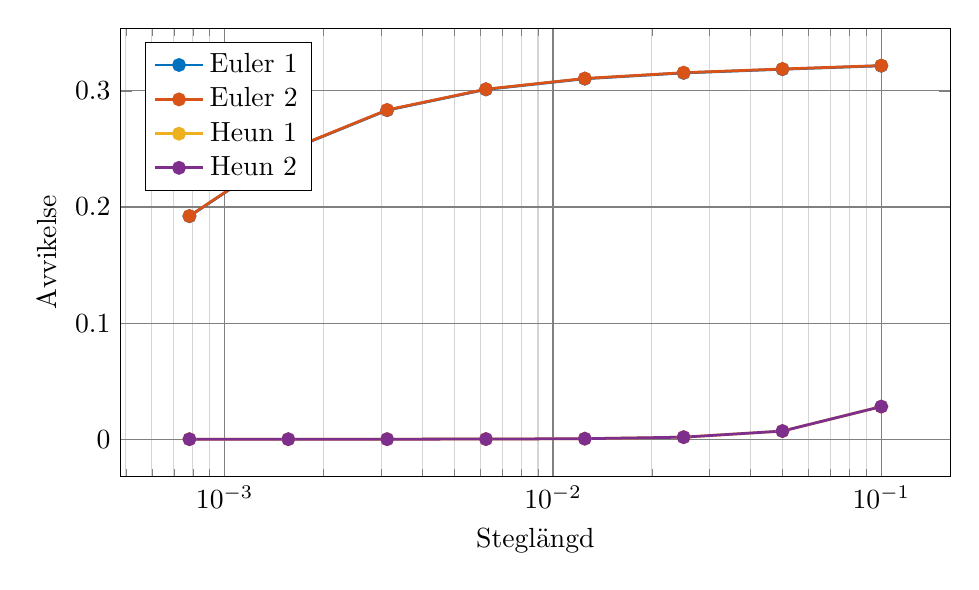
\begin{tikzpicture}
\definecolor{clr0}{RGB}{0, 114, 189}
\definecolor{clr1}{RGB}{217, 83, 25}
\definecolor{clr2}{RGB}{237, 177, 32}
\definecolor{clr3}{RGB}{126, 47, 142}
\definecolor{clr4}{RGB}{119, 172, 48}
\definecolor{clr5}{RGB}{77, 190, 238}
\definecolor{clr6}{RGB}{162, 20, 47}
\begin{axis}[xmode=log,xlabel=Steglängd,ylabel=Avvikelse,width=\textwidth,height=0.6\textwidth,grid=both,minor grid style={draw=gray!33},major grid style={draw=gray},legend pos=north west,]
\addplot[line width=1pt,mark=*,color=clr0] table {
0.1 0.3216494459631003
0.05 0.3186894419072372
0.025 0.3155010969579957
0.0125 0.31049018416633123
0.00625 0.3012748590142731
0.003125 0.28338033592678913
0.0015625 0.24870288610680347
0.00078125 0.19205471318320733
};
\addlegendentry{Euler 1}
\addplot[line width=1pt,mark=*,color=clr1] table {
0.1 0.32182413148025785
0.05 0.3188929312540557
0.025 0.31571520059551966
0.0125 0.31071411312749964
0.00625 0.3015083792157432
0.003125 0.2836216187385052
0.0015625 0.24894602478257977
0.00078125 0.19227553744928286
};
\addlegendentry{Euler 2}
\addplot[line width=1pt,mark=*,color=clr2] table {
0.1 0.02806777402191016
0.05 0.006998173827219515
0.025 0.0017494564488447339
0.0125 0.00043743784796757484
0.00625 0.00010937172693539481
0.003125 2.734459306542522e-05
0.0015625 6.836360888945041e-06
0.00078125 1.7091171581375127e-06
};
\addlegendentry{Heun 1}
\addplot[line width=1pt,mark=*,color=clr3] table {
0.1 0.028099570857876722
0.05 0.007005942549586446
0.025 0.0017514615598952226
0.0125 0.0004379469594839387
0.00625 0.00010950025374228245
0.003125 2.737688329134967e-05
0.0015625 6.844454521521976e-06
0.00078125 1.7111432057757987e-06
};
\addlegendentry{Heun 2}
\end{axis}
\end{tikzpicture}
        \caption{Inhomogen}
    \end{subfigure}

    \caption{Avvikelsen i system 7 för de olika funktionerna.}
    \label{fig:diagram_sys_7_errors}
\end{figure}

\subsection{System 8}
Den analytiska lösningen för system 8 är
\begin{equation*}
    \begin{cases}
        x=\frac{14139}{3029}(\frac{69}{82}\cos(\frac{\sqrt{3029t}}{10})+\frac{\sqrt{3029}}{82}\sin(\frac{\sqrt{3029t}}{10}))-\\
        \qquad \frac{73}{\sqrt{3029}}(\frac{\sqrt{3029}}{82}\cos(\frac{\sqrt{3029t}}{10})+\frac{69}{82}\sin(\frac{\sqrt{3029t}}{10}))-\frac{11565}{3029}\\
        \\[-7.5pt]
        y=\frac{14139}{3029}\cos(\frac{\sqrt{3029t}}{10})-\frac{73}{\sqrt{3029}}\sin(\frac{\sqrt{3029t}}{10})-\frac{11110}{3029}
    \end{cases}
\end{equation*}. Den motsvarande homogena differentialekvationen har lösningen 
\begin{equation*}
    \begin{cases}
        x=(\frac{69}{82}\cos(\frac{\sqrt{3029t}}{10})+\frac{\sqrt{3029}}{82}\sin(\frac{\sqrt{3029t}}{10}))-\\
        \qquad \sqrt{\frac{13}{233}}(\frac{\sqrt{3029}}{82}\cos(\frac{\sqrt{3029t}}{10})+\frac{69}{82}\sin(\frac{\sqrt{3029t}}{10}))\\
        \\[-7.5pt]
        y=\cos(\frac{\sqrt{3029t}}{10})-\sqrt{\frac{13}{233}}\sin(\frac{\sqrt{3029t}}{10})
    \end{cases}
\end{equation*}. En graf över olika steglängder och de associerade felen finnes i figur \ref{fig:diagram_sys_8_errors}.

\begin{figure}[h!]
    \centering

    \begin{subfigure}[h]{\textwidth}
        % Automatically generated code. github.com/ohman-emil/GA
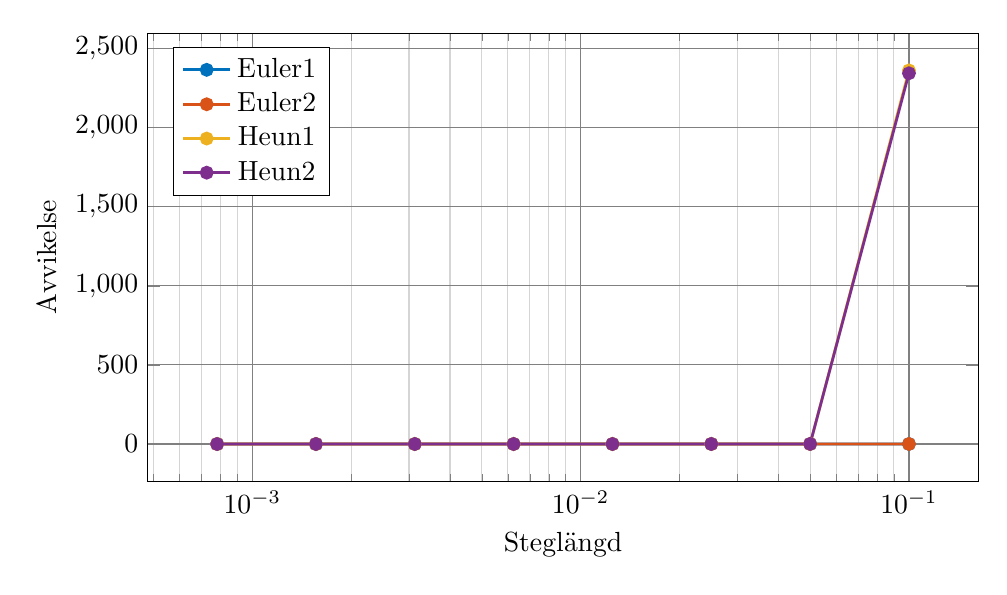
\begin{tikzpicture}
\definecolor{clr0}{RGB}{0, 114, 189}
\definecolor{clr1}{RGB}{217, 83, 25}
\definecolor{clr2}{RGB}{237, 177, 32}
\definecolor{clr3}{RGB}{126, 47, 142}
\definecolor{clr4}{RGB}{119, 172, 48}
\definecolor{clr5}{RGB}{77, 190, 238}
\definecolor{clr6}{RGB}{162, 20, 47}
\begin{axis}[xmode=log,xlabel=Steglängd,ylabel=Avvikelse,width=\textwidth,height=0.6\textwidth,grid=both,minor grid style={draw=gray!33},major grid style={draw=gray},legend pos=north west,]
\addplot[line width=1pt,mark=*,color=clr0,] table {
0.1 0.3176957254115023
0.05 0.3163097677803269
0.025 0.3136035779533316
0.0125 0.3082240625312869
0.00625 0.2975042859040087
0.003125 0.27611939100865307
0.0015625 0.23535684066729462
0.00078125 0.1742758902863571
};
\addlegendentry{Euler1}
\addplot[line width=1pt,mark=*,color=clr1,] table {
0.1 0.31695930668221933
0.05 0.3156618004189254
0.025 0.3130023871459322
0.0125 0.30763900508396985
0.00625 0.2969365961926278
0.003125 0.2755650245978292
0.0015625 0.23482315802408757
0.00078125 0.17381760385785275
};
\addlegendentry{Euler2}
\addplot[line width=1pt,mark=*,color=clr2,] table {
0.1 2361.428659795269
0.05 0.7311125264279719
0.025 0.27559284618314306
0.0125 0.069271418290286
0.00625 0.017267182183972118
0.003125 0.004314366283655049
0.0015625 0.0010785191129063806
0.00078125 0.0002696299115164901
};
\addlegendentry{Heun1}
\addplot[line width=1pt,mark=*,color=clr3,] table {
0.1 2343.3971867183886
0.05 0.7316102910407278
0.025 0.27526200520084043
0.0125 0.06924857517318879
0.00625 0.017267411534630614
0.003125 0.004314668543116661
0.0015625 0.001078592697633467
0.00078125 0.00026964608135362155
};
\addlegendentry{Heun2}
\end{axis}
\end{tikzpicture}
        \caption{Homogen}
    \end{subfigure}
    %
    \vspace{1em}\newline
    %
    \begin{subfigure}[h]{\textwidth}
        % Automatically generated code. github.com/ohman-emil/GA
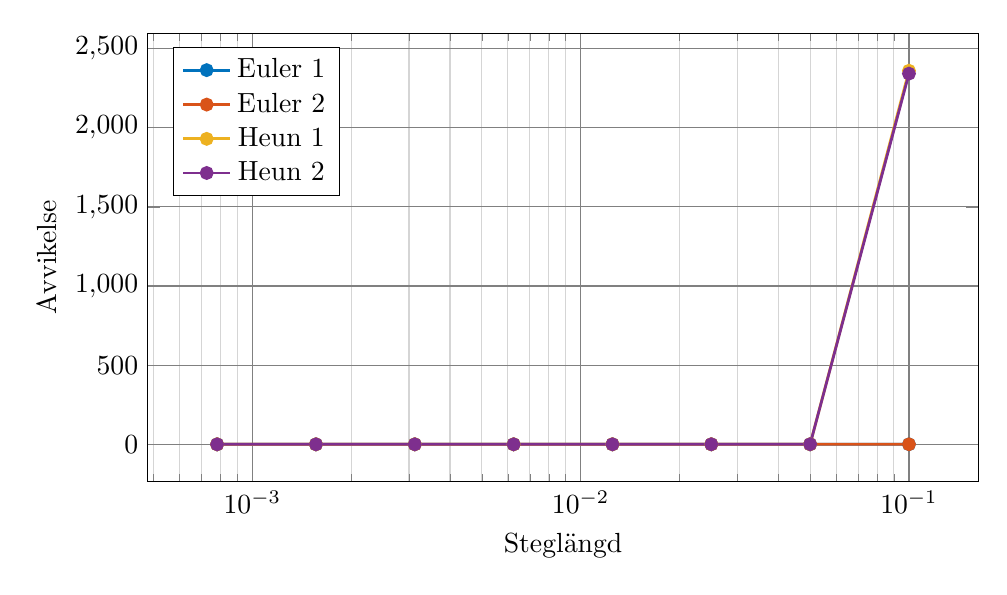
\begin{tikzpicture}
\definecolor{clr0}{RGB}{0, 114, 189}
\definecolor{clr1}{RGB}{217, 83, 25}
\definecolor{clr2}{RGB}{237, 177, 32}
\definecolor{clr3}{RGB}{126, 47, 142}
\definecolor{clr4}{RGB}{119, 172, 48}
\definecolor{clr5}{RGB}{77, 190, 238}
\definecolor{clr6}{RGB}{162, 20, 47}
\begin{axis}[xmode=log,xlabel=Steglängd,ylabel=Avvikelse,width=\textwidth,height=0.6\textwidth,grid=both,minor grid style={draw=gray!33},major grid style={draw=gray},legend pos=north west,]
\addplot[line width=1pt,mark=*,color=clr0] table {
0.1 0.3176776144730623
0.05 0.31629328080870855
0.025 0.3135911512832405
0.0125 0.30820385490000207
0.00625 0.2974833727320045
0.003125 0.27609704076729336
0.0015625 0.2353342787662127
0.00078125 0.17425605468448058
};
\addlegendentry{Euler 1}
\addplot[line width=1pt,mark=*,color=clr1] table {
0.1 0.31688808656869427
0.05 0.3156179456220494
0.025 0.31296376530555076
0.0125 0.307598423393
0.00625 0.2968971556158784
0.003125 0.2755249287859706
0.0015625 0.23478368068431818
0.00078125 0.17378330511036216
};
\addlegendentry{Euler 2}
\addplot[line width=1pt,mark=*,color=clr2] table {
0.1 2359.5900122340317
0.05 0.7311305536481064
0.025 0.27557101953059543
0.0125 0.06926644308699931
0.00625 0.017266243184902417
0.003125 0.0043141413312867945
0.0015625 0.0010784629803140481
0.00078125 0.000269615782021785
};
\addlegendentry{Heun 1}
\addplot[line width=1pt,mark=*,color=clr3] table {
0.1 2341.20052693826
0.05 0.7316512308482195
0.025 0.27524547697604385
0.0125 0.06925182078862971
0.00625 0.017268746980310962
0.003125 0.004315021197269691
0.0015625 0.0010786808965929991
0.00078125 0.00026966793622824913
};
\addlegendentry{Heun 2}
\end{axis}
\end{tikzpicture}
        \caption{Inhomogen}
    \end{subfigure}

    \caption{Avvikelsen i system 8 för de olika funktionerna.}
    \label{fig:diagram_sys_8_errors}
\end{figure}

\clearpage

\subsection{Skillnad mellan Eulers metod och Heuns metod}
Andelsskillnaden mellan Euler och Heuns metod för alla systemen finnes i figur \ref{fig:diff_euler_heun}. Andelsskillnaden räknades ut genom att dividera medelvärdet av avvikelsen i Heuns i de två funktionerna metod med medelvärdet av avvikelsen Eulers metod i de två funktionerna:
\begin{equation}
    \frac{\frac{1}{2}(H_1+H_2)}{\frac{1}{2}(E_1+E_2)}=\frac{H_1+H_2}{E_1+E_2}
\end{equation} där \(H_n\) är avvikelsen i Heuns metod för ekvation \(n\) och \(E_n\) är avvikelsen i Heuns metod för ekvation \(n\). Varje linje är således ett system. För system 5-8 användes de inhomogena ekvationerna.

\begin{figure}[h!]
    \centering
    % Automatically generated code. github.com/ohman-emil/GA
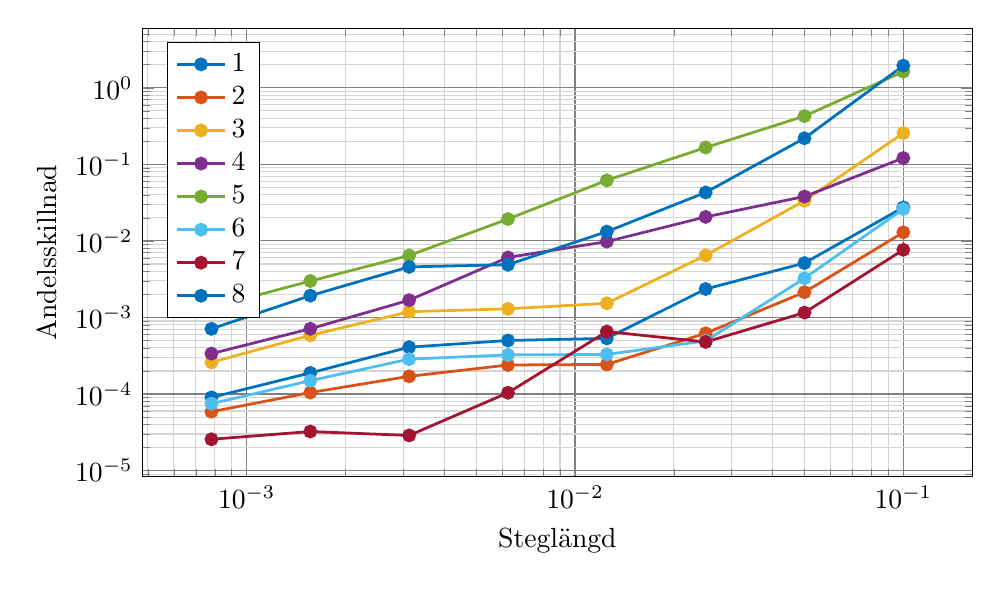
\begin{tikzpicture}
\definecolor{clr0}{RGB}{0, 114, 189}
\definecolor{clr1}{RGB}{217, 83, 25}
\definecolor{clr2}{RGB}{237, 177, 32}
\definecolor{clr3}{RGB}{126, 47, 142}
\definecolor{clr4}{RGB}{119, 172, 48}
\definecolor{clr5}{RGB}{77, 190, 238}
\definecolor{clr6}{RGB}{162, 20, 47}
\begin{axis}[xmode=log,ymode=log,xlabel=Steglängd,ylabel=Andelsskillnad,width=\textwidth,height=0.6\textwidth,grid=both,minor grid style={draw=gray!33},major grid style={draw=gray},legend pos=north west,]
\addplot[line width=1pt,mark=*,color=clr0] table {
0.1 0.027371900652614304
0.05 0.005134193726296163
0.025 0.0023547011523224457
0.0125 0.0005330309771963607
0.00625 0.0005002538942701676
0.003125 0.00040926434032323753
0.0015625 0.00018866621970747673
0.00078125 9.025619112498645e-05
};
\addlegendentry{1}
\addplot[line width=1pt,mark=*,color=clr1] table {
0.1 0.012935483489307962
0.05 0.002138928080102738
0.025 0.0006210549145464106
0.0125 0.000243406660920221
0.00625 0.00023932269725072592
0.003125 0.00017015067717236686
0.0015625 0.00010457325006417411
0.00078125 5.875236492113106e-05
};
\addlegendentry{2}
\addplot[line width=1pt,mark=*,color=clr2] table {
0.1 0.25570867072715087
0.05 0.033491343851594545
0.025 0.006465506424586497
0.0125 0.0015322023197099767
0.00625 0.0012959141359669658
0.003125 0.0011880202513032845
0.0015625 0.0005850731126304608
0.00078125 0.0002593253548676337
};
\addlegendentry{3}
\addplot[line width=1pt,mark=*,color=clr3] table {
0.1 0.12092533825709885
0.05 0.038016455135128
0.025 0.020582926852925596
0.0125 0.009791839286728013
0.00625 0.006082922500444976
0.003125 0.001682265150230636
0.0015625 0.0007113345611299891
0.00078125 0.00033666504966899016
};
\addlegendentry{4}
\addplot[line width=1pt,mark=*,color=clr4] table {
0.1 1.6253637284812188
0.05 0.4267403538795173
0.025 0.16586557907750896
0.0125 0.0618420398443939
0.00625 0.019316781367921917
0.003125 0.006449261308890801
0.0015625 0.0029901557975918016
0.00078125 0.0013522858138240942
};
\addlegendentry{5}
\addplot[line width=1pt,mark=*,color=clr5] table {
0.1 0.026093931201084566
0.05 0.0032496697338776246
0.025 0.0004941669972125922
0.0125 0.000328678256139826
0.00625 0.00032433538585313376
0.003125 0.0002854526357395255
0.0015625 0.00014933472384012268
0.00078125 7.477569924368722e-05
};
\addlegendentry{6}
\addplot[line width=1pt,mark=*,color=clr6] table {
0.1 0.007657656143286117
0.05 0.001156413232077404
0.025 0.0004782793328844254
0.0125 0.0006534314162330953
0.00625 0.00010383365348005192
0.003125 2.8752562551428965e-05
0.0015625 3.2342533825914594e-05
0.00078125 2.5625453429318645e-05
};
\addlegendentry{7}
\addplot[line width=1pt,mark=*,color=clr0] table {
0.1 1.9453521486609155
0.05 0.21938579470306932
0.025 0.042958950735964826
0.0125 0.013225074702565672
0.00625 0.004887274406225211
0.003125 0.004576229225490452
0.0015625 0.0019268765127308895
0.00078125 0.0007102133320153945
};
\addlegendentry{8}
\end{axis}
\end{tikzpicture}
    \caption{Andelsskillnaden mellan Eulers metod och Heuns metod.}
    \label{fig:diff_euler_heun}
\end{figure}
